\chapter{Predicting The Prices of Cryptocurrencies}\label{predictingpricesch}

Contrary to the title of this chapter, the price of cryptocurrencies, or any currency for that matter, cannot absolutely be predicted. One can however make an educated guess based on a variety of factors as to whether the price will rise or fall, or how severe a change in price will be. In this chapter, we will consider the various influencing factors in prices of cryptocurrency, followed by an examination of some existing methods of attempting to decipher a trend in cryptocurrency prices.

\section{The Volatility of Cryptocurrency}
As outlined in \textit{\ref{btcsec}: A Focus on Bitcoin}, the prices of cryptocurrency can be extremely unstable. For example, data taken from from CoinDesk \cite{coindeskprices} on April 12 2018, shows that in the space of one hour (11:00-12:00 GMT) the price of Bitcoin spiked from just under \$7000 to just under \$8000. There are countless of occurrences of this happening throughout the lifetime of Bitcoin. Another example of this volatility is when the currency reached its highest price on December 16 2017 of over \$19,300, before plummeting to \$13,800 a mere five days later - a drop of almost 30\%. It is the sheer instability of cryptocurrency prices and the rate at which they change that determines there will never be a dependable method of predicting prices.

However, one can take into account a variety of things when considering buying or selling cryptocurrency to determine if the time is right. It is important to clarify that the price is solely governed by demand, but there are indeed a great number of factors which may indirectly influence the price of cryptocurrency.

\subsection{Influencing Factors in Cryptocurrency Prices}\label{secinfluenceprices}
Traditional currencies are influenced by many things, such as warfare, political instability, and national debt. In contrast, there is only one direct cause for a change in the price of any cryptocurrency, and that is demand. While demand is the only thing that directly affects cryptocurrencies, many things influence the current level of demand.

\subsubsection{Price of Bitcoin}
Due to its popularity, the price of Bitcoin often affects the price of other cryptocurrencies. One could argue that if the price of Bitcoin is affected by the same events as other cryptocurrencies, its prices will change in tandem with those of other cryptocurrencies. However, the size and popularity of Bitcoin lead many to look to its data when considering buying or selling any cryptocurrencies. 

For example, consider a sudden increase in negative media content related to Blockchain technology. If the majority agree with the negative content, the majority of the market could decide to sell their investments. Bitcoin, with an estimated market dominance of 40-45\% \cite{coinmarketcap}, also the majority, would subsequently decline in price. If most of the majority sold their Bitcoin, owners of other cryptocurrencies would be likely to sell due to the majority of the market declining.   

By comparing graphed data of the prices of a given cryptocurrency against those of Bitcoin, it becomes clear that Bitcoin activity does in fact have a bearing on other cryptocurrency prices. See \textit{Figure \ref{prices1w}} below, detailing the prices of Bitcoin and Ethereum over one week.

\begin{figure}[h]
    \centering
    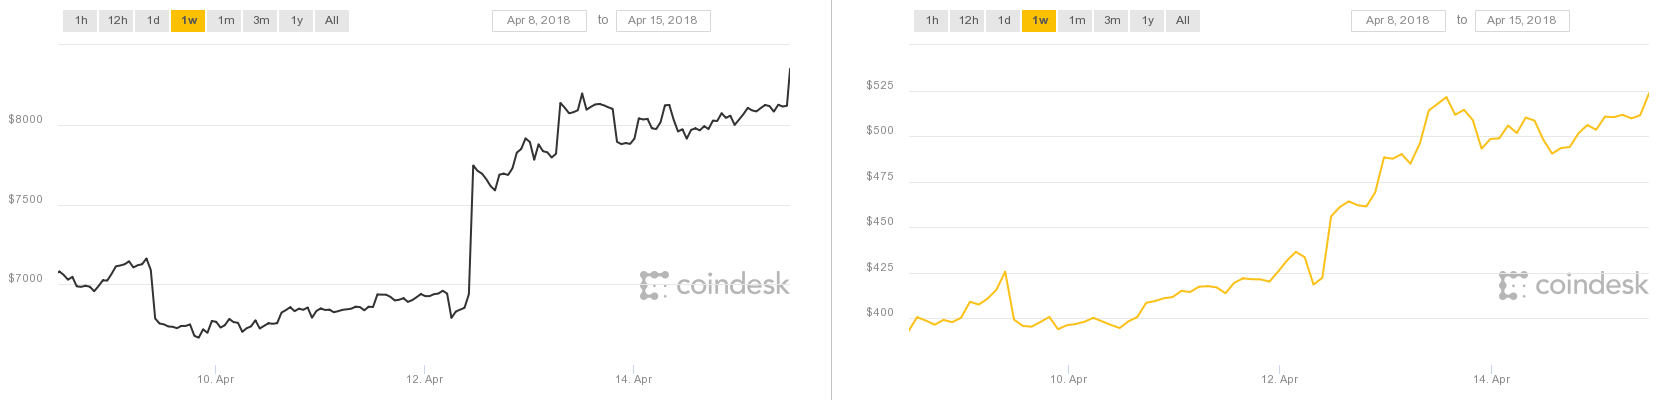
\includegraphics[width=\textwidth, keepaspectratio]{pricecharts/btceth1W.png}
    \caption{BTC and ETH Prices, Apr 8 - 15 2018 \cite{coindeskprices}}
    \label{prices1w}
\end{figure}    

While one could consider this purely coincidence, with a week arguably not being long enough to decipher any relationships between the two, the same can also been seen for a longer period of three months. Consider \textit{Figure \ref{prices3m}} below.

\newpage

\begin{figure}[h]
    \centering
    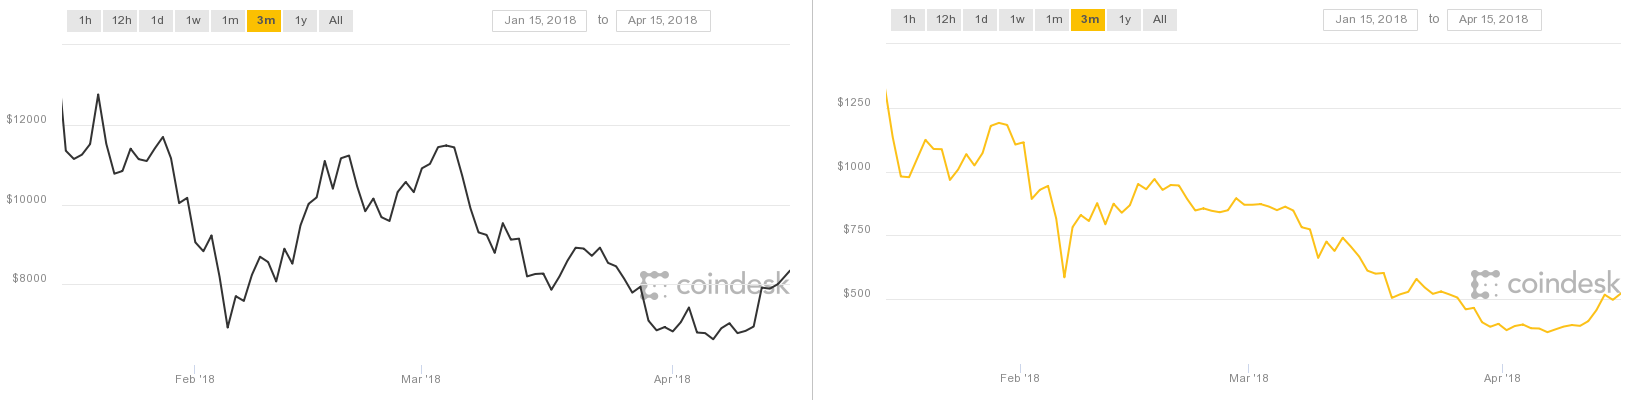
\includegraphics[width=\textwidth, keepaspectratio]{pricecharts/btceth3M.png}
    \caption{BTC and ETH Prices, Jan 15 - Apr 15 2018 \cite{coindeskprices}}
    \label{prices3m}
\end{figure}

In both instances, the prices of both Bitcoin and Ethereum follow roughly the same path. Bitcoin prices can be seen to be much more volatile, rising and falling more severely and in shorter spaces of time than Ethereum prices. For example, one should consider the sharp rise in price of Bitcoin shortly after April 12, 2018 against the slightly more dulled rise of Ethereum. This can also be observed in the rise and fall of the prices from Febrary to March 2018; the price of Bitcoin is seen to be more erratic, detailing many sudden increases and decreases. Ethereum follows the same general path with less sharp changes, implying that Bitcoin does lead to increased buying or selling of Ethereum. 
  
\subsubsection{Hyperbole Across the Media}
As introduced above, media content can often play a large role in the changing of currency prices. Of course, it is hard to effectively quantify the effect of social media coverage by simply observing prices on a graph.

In a very recent article, Mai et al found that social media in particular can be a relatively accurate predictor of future Bitcoin prices \cite{socmedimpact}. Focusing on one of the more popular forums for discussing Bitcoin, \textcolor{NavyBlue}{\url{bitcointalk.org}}, Mai et al concentrated on forum posts over three years, from 1 January 2012 to 31 December 2014. Data was also obtained from \textcolor{NavyBlue}{\url{Twitter.com}}, in the form of tweets containing the \textcolor{NavyBlue}{\href{https://twitter.com/hashtag/bitcoin?lang=en}{\#Bitcoin}} hashtag.

By using natural language processing to determine the number of positive or negative posts, Mai et al carried out tests on the obtained data through the use of vector error correction models to detect any interdependencies between pricing and social media coverage. Based on extensive testing as outlined in \cite{socmedimpact}, Mai et al found that social media activity is in fact at least a partial indicator or future Bitcoin prices.

Concluding their findings, Mai et al also highlight the issue of silent majority, vocal minority; in that most social media uses simply observe content as opposed to actively discussing the content. While this of course will skew results, the authors found this issue to be less common in the specified forum as opposed to Twitter. The group therefore concluded based on tests that any sentiments expressed on a forum have a bigger bearing on Bitcoin prices than those expressed on Twitter.

\subsection{The Bitcoin Bubble}
A bubble, defined as \textit{"a state of booming economic activity that often ends in a sudden collapse"} \cite{bubbledef}, is a term commonly used in conversations across a variety of finance-related conversations. Often referring to a very lucrative or advantageous period of time, these occurrences rarely last long, often "popping" suddenly as a physical bubble would.

\subsubsection{Historic Similarities}
The world has seen many bubbles end badly in the last 20 years, most notably "The Great Recession" which began in late 2007 \cite{greatrecession}. Prior to this downturn, the economy of the developed world had enjoyed great success financially, with financial institutions fuelling this by offering increased levels of loans and mortgages. 

While there are ongoing arguments as to whether Bitcoin is a bubble or not, and what the severity of a possible crash will be in the event that it is, it is hard to definitively agree with one argument or another. Any bubble in regards to Bitcoin would be brought on much differently to that of The Great Recession, and would likely run its course and recover differently to how the world economy recovered from The Great Recession. There are substantially more influences in the activity of the world economy than there are for any cryptocurrency activity, the prices of which are governed solely by demand.

One example of a historic bubble which has been likened to the popularity seen by Bitcoin is that of the "tulip mania" bubble experienced by the Netherlands in the 1600s. While the tulip mania bubble was not as disastrous or as widespread as is commonly believed, it did leave many merchants in debt. Similarly, if Bitcoin were to collapse tomorrow, only those who had invested would be affected and not the national or international economy. Unlike tulips however, Bitcoin does have core uses outside of simply existing; it can be used as a transferable asset, as well as a store of value \cite{tulipmania}. 
\subsubsection{The Future of Bitcoin}
Of course, with such a volatile asset as Bitcoin, it is hard to say if any major collapse will ever occur, or if prices would ever recover from such a collapse. Any possible collapse of Bitcoin could occur for a number of reasons, such as the advent of quantum computers capable of compromising the blockchain, or a simple sudden loss of faith in the resource.

The initial years of Bitcoin saw a relatively stable increase in prices, slowly climbing to just under \$1000 by the end of 2016 \cite{coindeskprices}. It is clear this growth in price was fuelled by a gradual, natural growth of Bitcoin's popularity, easily seen by exploring the popularity of the term in Google searches over time \cite{googletrendbtc}. For most of its life, Bitcoin had been a relatively unknown term, or at least certainly not understood by the majority. In 2017 however, the term began to gather momentum are prices surpassed the \$1000 mark, with prices rising exponentially for the duration of 2017. At Bitcoin's peak of \$19,661.63 on 17 December 2017 \cite{coindeskprices}, prices had risen by a staggering 1870\% in one single year. While there is no concrete calculation that can be done to determine what actually qualifies as a bubble, the sharp, almost irrational growth of prices would be difficult to refer to as anything other than a bubble. In keeping with the characteristics of every boom and bust cycle, Bitcoin suddenly plummeted to \$13,857.14 on 22 December 2017. In the months since, prices have continued to rise and fall toward an overall gradual decline, which could be interpreted as simply a correction of the ridiculous prices to prices that reflect more accurately the cryptocurrency's worth, as opposed to an actual crash. 

As very recently summarised well by Derousseau in \cite{airoutbubble}, factors such as increased interest by governments, the arrival of Bitcoin futures, and the growing number of alternative cryptocurrencies could all be leading factors in price declines. Bitcoin has now been banned by governments in a number of countries, which of course negatively affects the market as those countries' residents sell of their currency. Bitcoin futures, allowing investors to simply bet on whether Bitcoin prices will rise or fall, means that those interested in cryptocurrency no longer need to own that currency in order to profit from it, possibly leading to a decline in the market in future. Lastly, as more cryptocurrencies are added to the market, the market space for existing currencies reduces. While popularity of the bigger currencies may remain steady, the addition of newer varieties is likely to steal some of the spotlight from Bitcoin as people invest early with the hopes of these new currencies eventually reaching Bitcoin prices.

To conclude, the volatility of Bitcoin prices and cryptocurrency prices in general determines that one will likely never be able to accurately predict the price changes of these currencies. While Bitcoin itself may have gone through a bubble-like phase in 2017 and early 2018, its stabilisation is unlike that of a national economy after a financial crash. Perhaps Bitcoin will continue on a path similar to that of the last year, rising and falling but remaining in the order of thousands of dollars per coin. Perhaps interest and ultimately faith in Bitcoin will dwindle, resulting in the outright collapse of the currency. Nonetheless, it would be absolutely absurd to claim one or the other will definitely occur - we are simply going to have to observe these events as they happen.

\section{Deciphering Trends in Prices}
It is with this knowledge in mind that we progress to the applied aspect of this project. As examined above, there is no method to accurately predict the prices of any cryptocurrency. However, there are certainly trends in prices, which can be examined and attempted to be forecast using a variety of new technologies. 

Building on the information discussed in this and previous chapters, we will now examine the applied element of this project; a web application for displaying Bitcoin prices against the Euro and predicting future values of Bitcoin. 

It should be noted that while the web application was designed to be as easily understood as possible, it is still encouraged that the user has at least partly read and understood the preceding chapters of this dissertation.
